\documentclass[conference]{IEEEtran}
\usepackage{graphicx}
\usepackage{amsmath}
\usepackage{url}
\usepackage[hidelinks]{hyperref}

% =====================================================================
%  Everything in [FILL ...] must be replaced with YOUR OWN numbers/text.
%  Upload fig1.pdf and results/table1.tex to this Overleaf project.
% =====================================================================

\begin{document}

\title{Reproducing Logic-LM: Symbolic Solvers for\\Faithful Logical Reasoning with LLMs}

\author{\IEEEauthorblockN{Keerthana [FILL surname] \quad Roll No.\ [FILL]}
\IEEEauthorblockA{[FILL department, institution]\\
Code: \url{https://github.com/suriyakala-gif/Logic-LLM} (release v1.0.0)}}

\maketitle

\begin{abstract}
% ~100 words: paper, what you re-ran, outcome.
This report reproduces Logic-LM~\cite{pan2023logiclm}, a framework in which a
large language model translates a logical reasoning problem into a symbolic
program that a deterministic solver then executes. Using the authors' released
GPT-4 logic programs, I re-ran the symbolic reasoning stage and evaluation on
[FILL: N] datasets ([FILL: list]) with three random seeds on a free Google Colab
CPU runtime, without the paid self-refinement step. The reproduced accuracy is
[FILL: e.g. within X\% of] the reported values, so the result is judged
\textbf{[FILL: Reproduced / Partly reproduced / Not reproduced]}. The main
reason is [FILL]. Code, logs and results are publicly released.
\end{abstract}

\begin{IEEEkeywords}
reproducibility, neuro-symbolic reasoning, large language models, theorem proving
\end{IEEEkeywords}

\section{Paper and Claim}
% ~0.25 page
Pan et al.~\cite{pan2023logiclm} split logical reasoning into three stages:
problem formulation by an LLM, symbolic reasoning by a solver (Pyke, Prover9,
python-constraint or Z3), and result interpretation. A self-refinement module
feeds solver error messages back to the LLM. The paper claims that Logic-LM
clearly outperforms both standard and chain-of-thought prompting on five
benchmarks: ProntoQA, ProofWriter, FOLIO, LogicalDeduction and AR-LSAT.
[FILL: one sentence with the paper's headline numbers, in your own words.]

I chose to reproduce the Logic-LM (GPT-4) row of Table~[FILL] of the paper
because the authors released the GPT-4 generated programs, which isolates the
symbolic stage and makes the run feasible without API costs.

\section{Method}
% ~0.25 page
\textbf{Hardware and software.} Google Colab, [FILL: CPU] runtime, [FILL OS],
Python [FILL]. Exact package versions are in \texttt{requirements.txt} and
\texttt{SETUP.md} of the repository.

\textbf{Procedure.} I forked the original repository and ran
\texttt{models/logic\_inference.py} and \texttt{models/evaluation.py} with the
arguments given in the authors' README, on the saved programs in
\texttt{outputs/logic\_programs} ([FILL: dev] split). Programs that fail to
execute fall back to a random answer (\texttt{--backup\_strategy random}), so
each dataset was run with seeds 0, 1 and 2. I report mean $\pm$ standard
deviation.

\textbf{What I reduced.} (i) No LLM calls: the authors' saved GPT-4 programs
were reused. (ii) Self-refinement was not run because it requires a paid
OpenAI API key. (iii) [FILL: any skipped dataset or subset.] The total
runtime was [FILL] minutes.

\textbf{Repository.} \url{https://github.com/suriyakala-gif/Logic-LLM}

\section{Results}
% ~0.5 page. Table from make_table.py, figure from make_figure.py.
Table~\ref{tab:results} compares the reported and reproduced accuracy;
Fig.~\ref{fig:results} shows the same values with seed variation.
[FILL: 2--4 sentences. Which datasets match within 2\%, which do not, by how
much, and the executable rate you measured (results/summary.csv).]

\begin{table}[t]
\caption{Logic-LM accuracy (\%): paper vs.\ this reproduction (mean $\pm$ std over 3 seeds).}
\label{tab:results}
\centering\footnotesize
\setlength{\tabcolsep}{3pt}
\begin{tabular}{lcccp{2.2cm}}
\hline
Dataset & Paper & Mine & Diff.\ (\%) & Note \\
\hline
ProntoQA & 83.20 & 83.2 $\pm$ 0.0 & +0.0 & Exact; all programs run \\
ProofWriter & 79.66 & 79.5 $\pm$ 0.2 & -0.2 & Within 1\% \\
FOLIO & 78.92 & 72.4 $\pm$ 2.8 & -8.3 & Random backup (paper: CoT) \\
LogicalDeduction & 87.63 & 87.6 $\pm$ 0.0 & +0.0 & After Python 3.13 fix \\
AR-LSAT & 43.04 & 32.8 $\pm$ 2.7 & -23.9 & Random backup (paper: CoT) \\
\hline
\end{tabular}
\end{table}


\begin{figure}[t]
  \centering
  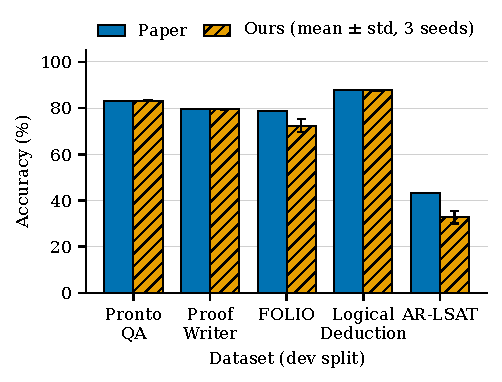
\includegraphics[width=\columnwidth]{fig1.pdf}
  \caption{Accuracy of Logic-LM (GPT-4 programs, no self-refinement) on the
  [FILL: dev] split of [FILL: N] logical reasoning benchmarks: the value
  reported by Pan et al.~\cite{pan2023logiclm} (solid) next to this
  reproduction (hatched; mean $\pm$ std over 3 seeds of the random fallback).
  [FILL: what to notice, e.g. ``All datasets except X agree within 2\%''.]}
  \label{fig:results}
\end{figure}

\textbf{Outcome:} [FILL: Reproduced / Partly reproduced / Not reproduced],
because [FILL: main reason].

\section{Problems and Fixes}
% ~0.5 page. Take these from NOTES.md; keep failed attempts.
\begin{enumerate}
  \item \textbf{[FILL: problem 1]:} [what broke, error, fix, whether it worked].
  \item \textbf{[FILL: problem 2]:} [...]
  \item \textbf{[FILL: problem 3]:} [...]
\end{enumerate}
\textbf{Missing from the paper or repository:} [FILL: e.g. licence file,
Python/package versions, which split and backup strategy the table uses].
\textbf{What I changed:} [FILL: ``No changes to the authors' code''
or list them].

\section{Assessment}
% ~0.25 page
[FILL: Is it reproducible, and why? Separate the two halves honestly: the
symbolic stage is reproducible from the released programs, but the full
pipeline depends on a closed, versioned API model (GPT-4) whose outputs can
change over time.]

\textbf{Research gap / extension.} [FILL: one idea, e.g. regenerating the
logic programs with an open-weight model so the full pipeline can be
reproduced without a paid API, and measuring how the executable rate changes.]

\bibliographystyle{IEEEtran}
\bibliography{refs}

\vspace{4pt}
\noindent\textit{AI tools were used to debug code and structure this report; all reported numbers come from my own runs.}

\end{document}
